\section{Options to Compute SVD.}

\begin{itemize}
\item Given input covariance matrix $\bM$, use \textbf{Eigen Decomposition} or \textbf{Singular Value Decomposition (SVD)} Operation as forward computation, and use the analytic solution of its gradient for backward propogation.
\item Given input covariance matrix $\bM$, vectors with random values $[\bv_1^{1}, \bv_2^{1}, ...]$, use \textbf{Power Iteration} as forward computation, and use its gradient for backward propogation.
\item Given input covariance matrix $\bM$, vectors with random values $[\bv_1^{1}, \bv_2^{1}, ...]$, use \textbf{Eigen Decomposition} or \textbf{SVD} Operation as forward computation, and use \textbf{Power Iteration} to approximate the analytic solutions of the gradient for backward propogation.
\end{itemize}

Usually, people choose either option 1 or option 2 to compute SVD, but both of them have problems.
In option 1, \textbf{Eigen Decomposition} or \textbf{Singular Value Decomposition (SVD)}, the analytic solutions of the gradient sometimes causes NaN problem when there are two or more eigenvalues are too close to each other.
In option 2, if the two eigenvalues are very close, eigenvectors could not be computed precisely with limited power iteration number. Thus, during backprorogation, the derivatives will be very inaccurate and destroy the parameters of model, and cause numerical instability in the training process.

In this paper, we propose to using option 3. During forward pass, we use \textbf{SVD} to compute the eigenvalues. 
SVD is numerically more stable than eigendecomposition \cite{nakatsukasa2013stable} as SVD implementation employs a divide-and-conquer strategy, while the eigendecomposition uses QR algorithm. 
During backpropogation, we employ \textbf{Power Iteration} method to compute the numerical solutions of the covariance matrix $\bM$ gradient.
In \textbf{sections} \ref{sec: pi} \& \ref{sec: mbp}, we will prove that when the iteration number goes to infinite, the accumulated gradients (\emph{i.e.} numerical solution) from the \textbf{Power Iteration} method is exactly the same with the analytic solution of the gradient.

\section{Approximate SVD gradient with Power Iteration in backpropogation}
In the following 2 subsections, we will prove that when the gradient computed from Power Iteration equals to the gradients computed from SVD.
	\subsection{Gradient of Power Iteration}
	\label{sec: pi}
	To compute the leading eigenvector $\bv$ of $\bM$, Power Iteration uses the following standard formula,
	\begin{equation}
	\bv^{(k)} = \frac{\bM\bv^{(k-1)}}{\| \bM\bv^{(k-1)} \|},
	\end{equation}
	in which $\| {\cdot} \|$ denotes the $l_2$ norm, and $v^{(0)}$ is usually initialized randomly with  $\|v^{(0)}\|{=}1$.
    Its gradient is as follows~\cite{ye2017dynamic},
	\begin{equation}
	\begin{aligned} 
	\frac{\partial L}{\partial \bM} &=\sum_{k} \frac{\left(\bI-\bv^{(k+1)} \bv^{(k+1)\top}\right)}{\left\|\bM \bv^{(k)}\right\|} \frac{\partial L}{\partial \bv^{(k+1)}} \bv^{(k)\top} \\
	\frac{\partial L}{\partial \bv^{(k)}} &=\bM \frac{\left(\bI-\bv^{(k+1)} \bv^{(k+1)\top}\right)}{\left\|\bM \bv^{(k)}\right\|} \frac{\partial L}{\partial \bv^{(k+1)}} 
	\end{aligned}
	\end{equation}

In the forward pass, we use SVD to compute the eigenvector, $\bv$.
If we feed $\bv$ directly to the power iteration method as initial value, we will have $\bv {=} \bv^{(0)} {\approx}\bv^{(1)} {\approx} \bv^{(2)}{\approx} \cdots {\approx}\bv^{(k)} \cdots {\approx}\bv^{(K)}$.
After introducing $\frac{\partial L}{\partial \bv^{(k)}}, \; k=1,2, \cdots, K$ into $\frac{\partial L}{\partial \bM}$, we can obtain
	\begin{equation}
	\frac{\partial L}{\partial \bM}
	 = \left( \frac{\left(\bI-\bv \bv^{\top}\right)}{\left\|\bM \bv\right\|}  +
	 \frac{\bM \left(\bI-\bv \bv^{\top}\right)}{\left\|\bM \bv\right\|^{2}}  + \cdots +
	 \frac{\bM^{K-1} \left(\bI-\bv \bv^{\top}\right)}{\left\|\bM \bv\right\|^{K}} \right) \frac{\partial L}{\partial \bv^{(K)}}
	\bv^{\top}
	\label{eq: pi_pytorch}
	\end{equation}	

The deduction details of Eq.\ref{eq: pi_pytorch} is available in the supplementary material.
Eq.\ref{eq: pi_pytorch} is the form we adopt to compute the gradients of SVD, and we set $K{=}19$.


\subsection{Relationship between Gradients of Power Iteration and SVD}
In this subsection, we are going to prove that the gradients of SVD and Power Iteration are equivalent. In the end of this section, we can observe that when the number of the iterations goes to infinity, the gradients of Power Iteration can be written as the same form as the one of SVD.
\subsubsection{Gradients of Power Iteration}
The gradients of Power Iteration could be formulated into another form using the following properties.
	\begin{equation}
	\begin{aligned}
	\bM & = \bV \Sigma \bV^{\top} & = & \lambda_{1}\bv_{1}\bv_{1}^{\top} + \lambda_{2}\bv_{2}\bv_{2}^{\top} + \cdots +  \lambda_{n}\bv_{n}\bv_{n}^{\top}, \\
	\bM^{k} & = \bV \Sigma^{k} \bV^{\top} & = & \lambda_{1}^{k}\bv_{1}\bv_{1}^{\top} +  \lambda_{2}^{k}\bv_{2}\bv_{2}^{\top} + \cdots + \lambda_{n}^{k}\bv_{n}\bv_{n}^{\top},\\
	\end{aligned}
	\label{eq: term_k}
	\end{equation}
	and $\left\|\bM\bv\right\| = \left\| \lambda \bv \right\|= \lambda$,
	in which $\bv = \bv_1$ is the leading eigenvector and $\lambda=\lambda_1$ is the leading eigenvalue.
	By introducing Eq.\ref{eq: term_k} into Eq.\ref{eq: final-form}, the derivative can be further formulated as
	
	\begin{equation}
	\begin{aligned} 
	\frac{\partial L}{\partial \bM}
	& =\left( \frac{\left(\bI-\bv_1 \bv_1^{\top}\right)}{\left\|\bM \bv_1\right\|}  +
	 \frac{\bM \left(\bI-\bv_1 \bv_1^{\top}\right)}{\left\|\bM \bv_1\right\|^{2}}  + \cdots +
	 \frac{\bM^{K-1} \left(\bI-\bv_1 \bv_1^{\top}\right)}{\left\|\bM \bv_1\right\|^{K}} \right)
	 \frac{\partial L}{\partial \bv_1^{(K)}}\bv_1^{\top} \\
	&=\left( \frac{\left(\bI-\bv_1 \bv_1^{\top}\right)}{\left\|\bM \bv_1\right\|} +
	\frac{\left(\bM-\lambda \bv_1 \bv_1^{\top}\right)}{\left\|\bM \bv_1\right\|^2}  + \cdots +
	\frac{\left(\bM^{K-1} - \lambda^{K-1}\bv_1\bv_1^{\top}\right)}{\left\|\bM \bv\right\|^{K}} \right) \frac{\partial L}{\partial \bv_1^{(K)}} \bv_1^{\top}\\
	&=\left( \frac{\left(\sum_{i=2}^{n}\bv_{i}\bv_{i}^{\top}\right)}{\lambda_1}      +
	\frac{\left(\sum_{i=2}^{n}\lambda_{i}\bv_{i}\bv_{i}^{\top}\right)}{ \lambda_{1}^{2}} +  \cdots +
	\frac{\left(\sum_{i=2}^{n}\lambda_{i}^{K-1}\bv_{i}\bv_{i}^{\top}\right)}{\lambda_{1}^{K}} \right) \frac{\partial L}{\partial \bv_1^{(K)}}
	\bv^{\top}\\
	&=\left(\sum_{i=2}^{n}\left(
	\frac{1}{\lambda_{1}} +
	\frac{1}{\lambda_{1}}\left(\frac{\lambda_{i}}{\lambda_{1}}\right)^{1} +
	\frac{1}{\lambda_{1}}\left(\frac{\lambda_{i}}{\lambda_{1}}\right)^{2} + \cdots +
	\frac{1}{\lambda_{1}}\left(\frac{\lambda_{i}}{\lambda_{1}}\right)^{K-1}
	\right)\bv_{i}\bv_{i}^{\top}
	\right)\frac{\partial L}{\partial \bv_{1}^{(K)}}\bv_{1}^{\top}\\
	\end{aligned}
	\label{eq: geo-prog-series}
	\end{equation}
	In Eq.\ref{eq: geo-prog-series}, we have a geometric progression series.
	Given that $${1 - (\frac{\lambda_{i}}{\lambda_{1}})^k \rightarrow 1}, \text{when} \; k\rightarrow\infty, \vert \frac{\lambda_{i}}{\lambda_{1}} \vert<1,$$
	then we have
	\begin{equation}
	\frac{1}{\lambda_{1}} +
	\frac{1}{\lambda_{1}}\left(\frac{\lambda_{i}}{\lambda_{1}}\right)^{1} +
	\frac{1}{\lambda_{1}}\left(\frac{\lambda_{i}}{\lambda_{1}}\right)^{2} + \cdots +
	\frac{1}{\lambda_{1}}\left(\frac{\lambda_{i}}{\lambda_{1}}\right)^{k-1} = \frac{\frac{1}{\lambda_{1}}(1- (\frac{\lambda_{i}}{\lambda_{1}})^k)} {1 - \frac{\lambda_{i}}{\lambda_{1}}} 
	\rightarrow  \frac{\frac{1}{\lambda_{1}}}
	{1 - \frac{\lambda_{i}}{\lambda_{1}}}, \text{when} \; k\rightarrow\infty.
	\label{eq: geo-prog-series-deduction}
	\end{equation}
	
	Introducing Eq.\ref{eq: geo-prog-series-deduction} to Eq.\ref{eq: geo-prog-series}, we can obtain	
	\begin{equation}
	\frac{\partial L}{\partial \bM}
	=\left(\sum_{i=2}^{n}\left(
	\frac{\frac{1}{\lambda_{1}}}
	{1 - \frac{\lambda_{i}}{\lambda_{1}}}
	\right)
	\bv_{i}\bv_{i}^{\top}
	\right)\frac{\partial L}{\partial \bv_{1}^{(k)}}\bv_{1}^{\top}
	=\left(\sum_{i=2}^{n}
	\frac{\bv_{i}\bv_{i}^{\top}}
	{\lambda_{1} - \lambda_{i}}
	\right)\frac{\partial L}{\partial \bv_{1}^{(k)}}\bv_{1}^{\top}
	\label{eq: final-form}
	\end{equation}
	
	\subsubsection{Matrix Back-propagation}
	\label{sec: mbp}
	Eq.\ref{eq: mb} shows the analytic soltions of the gradients of matrix back-propagation~\cite{ionescu2015matrix}.
	It could be further formulated as the following form:
	\begin{equation}
	\frac{\partial L}{\partial M}
	=\sum_{i=2}^{n}\frac{1}{\lambda_{1}-\lambda_{i}}\bv_{i}\bv_{i}^{\top}\frac{\partial L}{\partial \bv_{1}}\bv_{1}^{\top}
	+ \cancel{\frac{\partial L}{\partial \lambda_i}\bv_i\bv_i^{\top}}
	\label{eq: mb-pi-form}
	\end{equation}
   We avoid using eigenvalues in the forward pass by formulating it as a function of eigenvectors using the Rayleigh quotient $\frac{\bv^{\top} \bM \bv}{\bv^{\top}  \bv}$, such that it has no gradients, which means $\frac{\partial L}{\partial \Sigma}$ could be ignored. The deduction details of Eq.\ref{eq: mb-pi-form} is available in the supplementary material.

Now we have shown that the partial derivative of \emph{e.g.}, $\bv_1$ computed from Power Iteration and SVD share the same form when $k\rightarrow \inf$.
Similar deductions could be done for  $\bv_i, i=2,3,...$.
This justifies that we could use power iteration method during backpropogation to approximate the gradients of SVD, but we need to choose an approximate iteration number.

\subsection{Impact of the Number of Power Iterations}
\label{subsec: talyer-expansion}
The power iteration number $K$ has a fundamental influence to the approximated gradients. In fact, it controls the upper bond of the gradients.

Eq.\ref{eq: geo-prog-series} can be viewed as the geometric series expansion of Eq.\ref{eq: mb-pi-form}.
When the covarriance matrix is singular with two same eigenvalues $\lambda_1 = \lambda_i$, the gradients computed from Eq.\ref{eq: mb-pi-form} will go to $\pm \infty$ as the denominator is 0. However, Eq.\ref{eq: geo-prog-series} naturally brings an upper bond to avoid this problem as shown in the following deduction,

	\begin{equation}
	\begin{aligned}
	\frac{\partial L}{\partial M} & = \sum_{i=2}^{n}\frac{1}{\lambda_{1}-\lambda_{i}}\bv_{i}\bv_{i}^{\top}\frac{\partial L}{\partial \bv_{1}}\bv_{1}^{\top} \\
	&\approx \left(\sum_{i=2}^{n}\left(
	\frac{1}{\lambda_{1}} {+}
	\frac{1}{\lambda_{1}}\left(\frac{\lambda_{i}}{\lambda_{1}}\right)^{1} {+}
	\frac{1}{\lambda_{1}}\left(\frac{\lambda_{i}}{\lambda_{1}}\right)^{2} {+} \cdots {+}
	\frac{1}{\lambda_{1}}\left(\frac{\lambda_{i}}{\lambda_{1}}\right)^{K-1}
	\right)\bv_{i}\bv_{i}^{\top}
	\right)\frac{\partial L}{\partial \bv_{1}}\bv_{1}^{\top}
	\end{aligned}
	\end{equation}
	
	\begin{equation}
	\begin{aligned}
	\left\| \frac{\partial L}{\partial M} \right\|
	& \leq \left\| \sum_{i=2}^{n}\left(
	\frac{1}{\lambda_{1}} {+}
	\frac{1}{\lambda_{1}}\left(\frac{\lambda_{i}}{\lambda_{1}}\right)^{1} {+}
	\frac{1}{\lambda_{1}}\left(\frac{\lambda_{i}}{\lambda_{1}}\right)^{2} {+} \cdots {+}
	\frac{1}{\lambda_{1}}\left(\frac{\lambda_{i}}{\lambda_{1}}\right)^{K-1}
	\right)\bv_{i}\bv_{i}^{\top}
	\right\| \left\|  \frac{\partial L}{\partial \bv_{1}} \right\|  \left\|  \bv_{1}^{\top} \right\| \\
	& \leq \left\| \sum_{i=2}^{n}\left(
	\frac{1}{\lambda_{1}} {+}
	\frac{1}{\lambda_{1}} {+}
	\frac{1}{\lambda_{1}} {+} \cdots {+}
	\frac{1}{\lambda_{1}}
	\right)\bv_{i}\bv_{i}^{\top}
	\right\| \left\|  \frac{\partial L}{\partial \bv_{1}} \right\|  \left\|  \bv_{1}^{\top} \right\| \\
	 & \leq \sum_{i=2}^{n} \left\| 
	\frac{K}{\lambda_{1}}
	\bv_{i}\bv_{i}^{\top}
	\right\| \left\|  \frac{\partial L}{\partial \bv_{1}} \right\|  \left\|  \bv_{1}^{\top} \right\|  
	\leq \frac{nK}{\lambda_{1}} \left\|  \frac{\partial L}{\partial \bv_{1}} \right\|
	\end{aligned}
	\end{equation}

Till now, we have obtain the upper bound of $\left\| \frac{\partial L}{\partial M} \right\|$. However, if $\lambda_{1} = 0$, the upper bound will also become $\infty$. To avoid this, we do the following operation to the covariance matrix $\bM = \bM + \epsilon I$, in which $I$ is an identity matrix. As $\bM$ is a covariance matrix which is positive semi-definite, the eigenvalues of $\bM + \epsilon I$ can be guaranteed to be larger than $\epsilon$.
Thus, the upper bound can be written as 

\begin{equation}
	\begin{aligned}
	\left\| \frac{\partial L}{\partial (M+\epsilon I) } \right\|
	\leq \frac{nK}{\epsilon} \left\|  \frac{\partial L}{\partial \bv_{1}} \right\|
	\end{aligned}
\end{equation}
in which $n$ is the dimension of the matrix and $K$ is the power iteration number. In the following experiments, we set $\epsilon = 10^{-4}$, and $K=19$.
In the following, we will explain why $K$ is set to 19.

\subsection{Select Appropriate Power Iteration Number K}

\begin{figure}[!htb]
\begin{center}
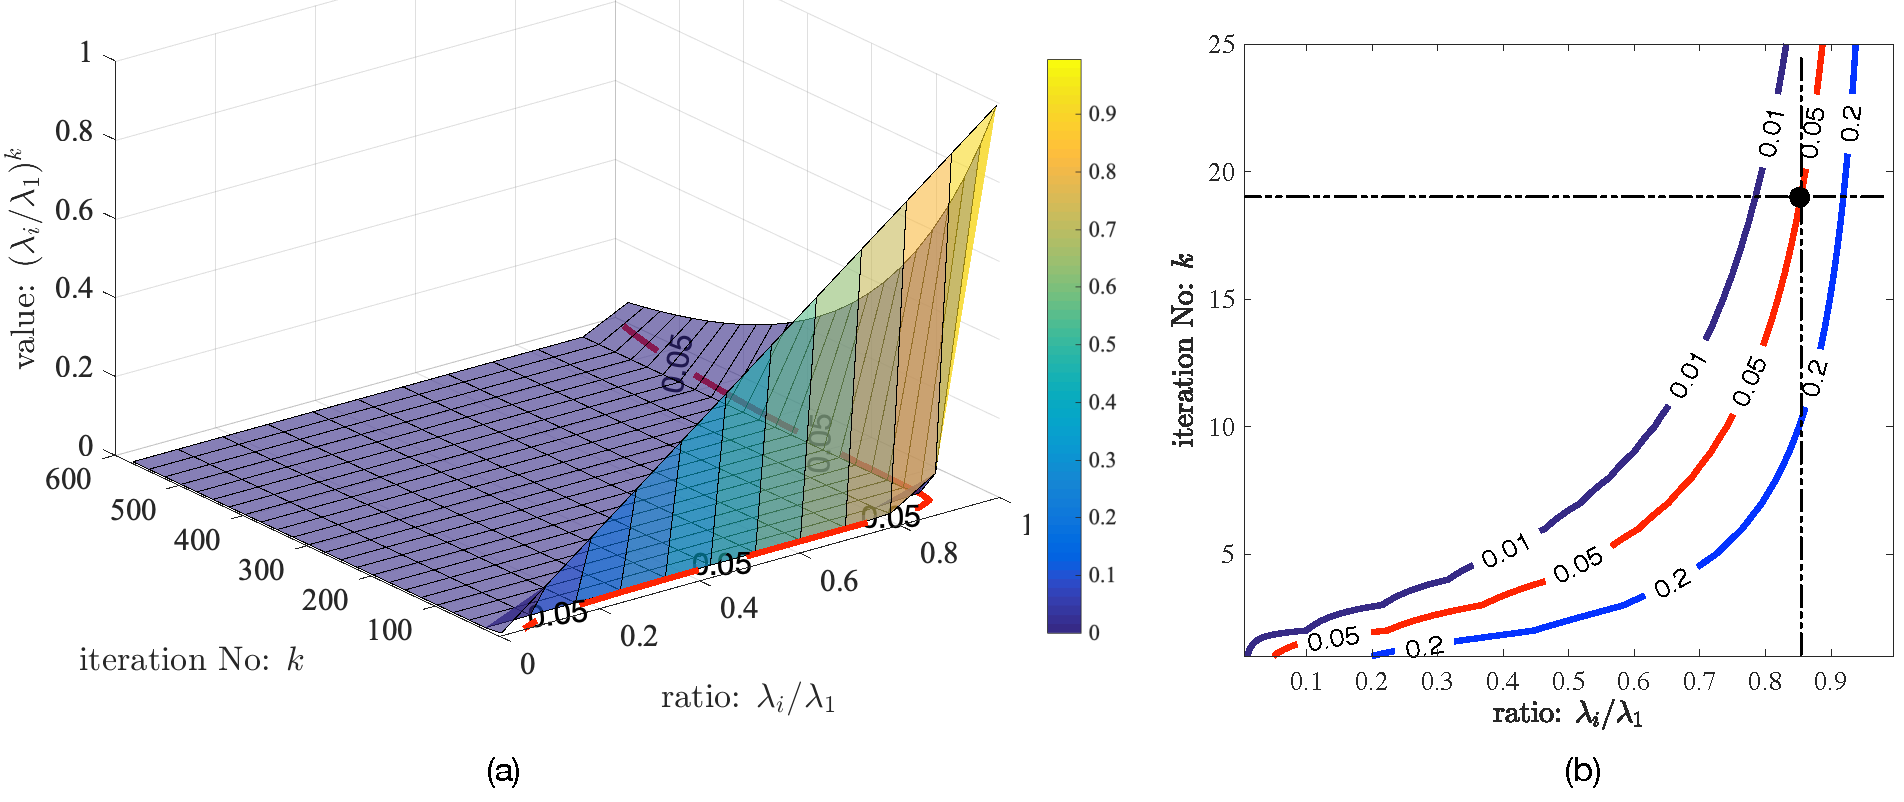
\includegraphics[width=\linewidth]{ratio-k.pdf}
\end{center}
\caption{(a) shows how the value of $(\lambda_k/\lambda_1)^k$ changes \emph{w.r.t.} the eigenvalue ratio $\lambda_k/\lambda_1$ and iteration number $k$. (b) shows the contour of curved surface in (a).}
\label{fig: curve}
\end{figure}

Fig. \ref{fig: curve} shows how the value of $(\lambda_i/\lambda_1)^k$ evolves with different power iteration number $k$ and ratio~$\lambda_i/\lambda_1$. We need to select appropriate $k$ for different $\lambda_i/\lambda_1$ given $(0 < \lambda_i/\lambda_1 \leq 1)$. 

Let's assume $(\lambda_i/\lambda_1)^k<0.05$ being a good approximation to $(\lambda_i/\lambda_1)^k=0$. Then we have
\begin{equation}
(\lambda_i/\lambda_1)^k<0.05 \Leftrightarrow k\; \text{ln}(\lambda_i/\lambda_1) < \text{ln}(0.05) \Leftrightarrow k \geq \frac{\text{ln}(0.05)}{\text{ln}(\lambda_i/\lambda_1)}.
\end{equation}
The minimum value of $k$ to satisfy $(\lambda_i/\lambda_1)^k<0.05$ is $k = \lceil \frac{\text{ln}(0.05)}{\text{ln}(\lambda_i/\lambda_1)} \rceil$.

\begin{table}[!htb]
\begin{centering}
\setlength\tabcolsep{4pt}
\begin{tabular}{ccccccccccccccc}
\hline
$\lambda_i/\lambda_1$ & 0.1& 0.2& 0.3 & 0.4 & 0.5 & 0.6 & 0.7 & 0.8 & \textbf{0.85} & 0.9 & 0.95 & 0.99 & 0.995 & 0.999 \\ \hline
$k = \lceil \frac{\text{ln}(0.01)}{\text{ln}(\lambda_i/\lambda_1)} \rceil $   & 2 & 2 & 3 & 4 & 5 & 6 & 9 & 14  & \textbf{19}   & 29  & 59   & 299  & 598   & 2995  \\ \hline
\end{tabular}
\caption{The minimum value of $k$ we need to guarantee $(\lambda_i/\lambda_1)^k<0.05$.}
\label{tab: kmin}
\end{centering}
\end{table}

Table \ref{tab: kmin} shows the minimum number of iterations we need to guarantee that the assumption holds. We can observe that when the two eigenvalues are very close to each other \emph{e.g.}, $\lambda_i/\lambda_1=0.999$, we need about 3000 iterations to achieve a good approximation. However, in practice, the case is very rare, and we set power iteration number to be 19. This will satisfy most of the cases. Besides, two very close eigenvalues usually leads to overflow according to Eq.\ref{eq: final-form} as the denominator $\lambda_1 - \lambda_i$ would be close to 0, but with our approximation, this problem could be avoided, and our method is more numerical stable.

\subsection{Practical Issues}
There are several practical issues when use Power Iteration to approximate the gradients of SVD.
In practice, take ZCA whitening for example, we use the following steps to compute the forward pass.

\begin{algorithm}[H]
 \KwData{$\mu=Avg(X)$, $\widetilde{X}=X-\mu$, $\bM=\widetilde{X}\widetilde{X}^{\top}+\epsilon I$, ($X \in R^{c\times nhw}$);}
 \KwResult{$V^{\top}\Lambda V=SVD(\bM)$; $\Lambda = diag(\lambda_1, \lambda_2, ..., \lambda_n)$; $V=\left[\bv_1,\bv_2,\cdots, \bv_n\right]$; $\gamma_i=\frac{\sum_{k=1}^i\lambda_k}{\sum_{k=1}^n\lambda_k}$; }
 initialization:$running_{\mu}=0$, $running_{S}=I$, $\widetilde{\bM} = \bM$,  $rank=1$\; 
 \For{$i=1:n$}{
  $\bv_i$ = Power Iteration($\widetilde{\bM}, \bv_i$);
  $\widetilde{\lambda_i} = \frac{\bv_i^{\top}\widetilde{\bM}\bv_i}{\bv_i^{\top}\bv_i}$;
  $\widetilde{\bM} = \widetilde{\bM} -  \widetilde{\bM}\bv_i\bv_i^{\top}$\;
  \eIf{$\lambda_i \leq \epsilon$  or  $\frac{\left| \widetilde{\lambda_i}-\lambda_i \right|}{\lambda_i} \geq 0.1$  or  $\gamma_i \geq (1-0.0001)$}{
   break\;
   }{$rank = i$, $\widetilde{\Lambda} = [\widetilde{\lambda_1}, \cdots, \widetilde{\lambda_i}]$.}
   }
   {truncate eigenvector matrix: $\widetilde{V}=[\bv_1, \bv_2, \cdots, \bv_{rank}]$
   compute subspace: $S=\widetilde{V}(\widetilde{\Lambda})^{-\frac{1}{2}}\widetilde{V}^{\top}$\;
   compute ZCA output: $X=S\widetilde{X}$\;
   update $running_{S} = momentum \cdot S + (1-momentum) \cdot running_{S}$\;
   update $running_{\mu} = momentum \cdot \mu + (1-momentum) \cdot running_{\mu}$\;
   }

 \caption{Forward Pass of ZCA whitening in Practice.}
 \label{alg: svd-foward}
\end{algorithm}


The first issue is that in the forward pass, the eigenvalues computed using SVD may be inaccurate.
Remember that to increase the stability, a small value $\epsilon$ is added to the diagonal axis of the covarraince matrix.
In this way, all the eigenvalues should be greater or equal to $\epsilon$. However, this is not the case when we use float precision instead of double precision.
To solve this problem, we employ truncated SVD.
When we found that the computed eigenvalue $\lambda_i \leq \epsilon$, we will truncate this $\lambda_i$ and its following $\lambda_{i+1}, \cdots,\lambda_{n}$.

The second issues is the approximation of the eigenvalues computed using $\widetilde{\lambda_i} = \frac{\bv^{\top} \widetilde{\bM} \bv}{\bv^{\top}\bv}$.
Because of the round-off error from $\widetilde{\bM} = \widetilde{\bM} -  \widetilde{\bM}\bv_i\bv_i^{\top}$, $\widetilde{\lambda_i}$ may be inaccurate and sometimes may be negative.
To avoid using incorrect eigenvalues, we also need to truncate it.

These two practical issues are the breaking conditions $\lambda_i \leq \epsilon$, $\frac{\widetilde{\lambda_i}-\lambda_i}{\lambda_i} \geq 0.1$ defined in Alg.\ref{alg: svd-foward}. Besides, we have added another constraint $\gamma_i \geq (1-0.0001)$ which means if the remaining energy preserved in $\widetilde{\bM}$ is less than 0.0001, we will also do the truncation as the remaining information is too trivial.